\begin{figure}[tb]
	\centering
	\begin{subfigure}{.49\columnwidth}
		\centering
		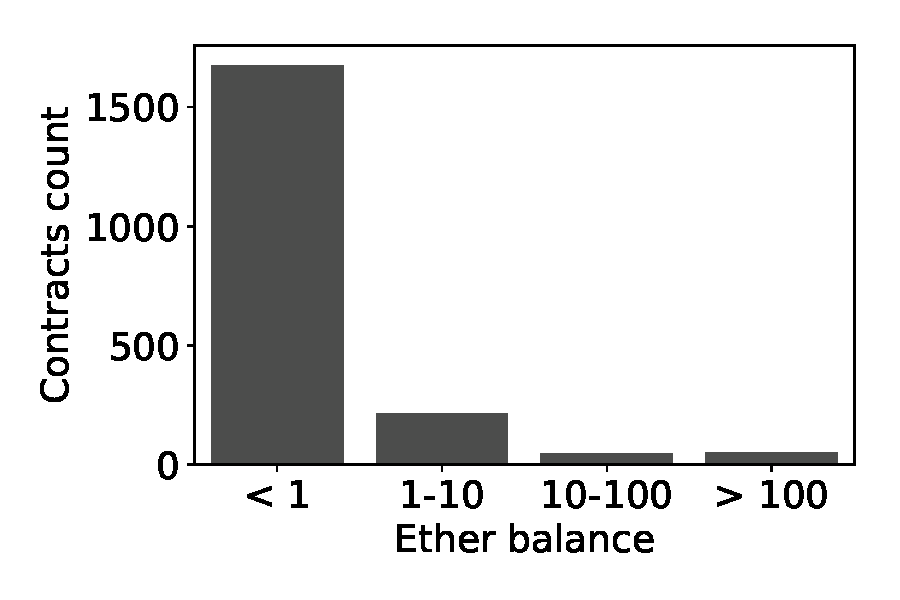
\includegraphics[width=\textwidth]{./5a-smart-contract-security/figures/balance-histogram.pdf}
		\caption{\scriptsize Ether held by contracts in our dataset\\with non-zero balance.}
		\label{fig:eth-held}
	\end{subfigure}
	\begin{subfigure}{.49\columnwidth}
		\centering
		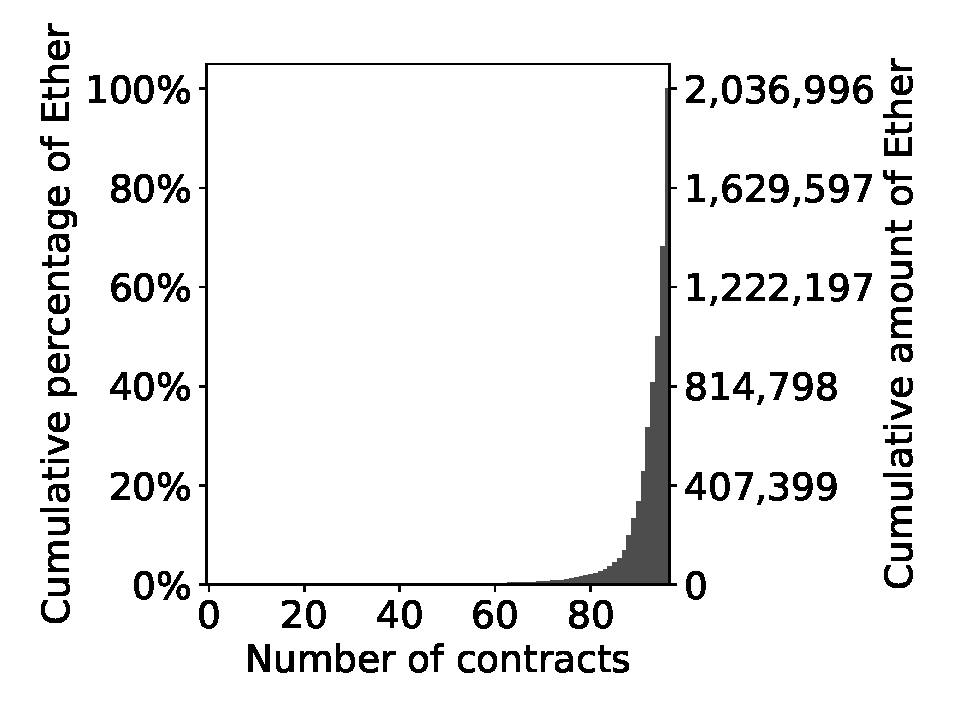
\includegraphics[width=\textwidth]{./5a-smart-contract-security/figures/cumulative-ether.pdf}
		\caption{\scriptsize Cumulative Ether held in the 96\\contracts in our dataset containing at least 10 ETH.}
		\label{fig:cumulative-eth}
	\end{subfigure}
	\caption{Ether held in contracts: describing the distribution.}
\end{figure}

\subsection{Discussion}
\label{sec:5a:discussion}

Even considering the limitations of our system, it is clear that the exploitation of smart contracts is vastly lower than what could be expected. In this section, we present some of the factors we think might be impacting the actual exploitation of smart contracts.

% \subsection{Contracts holding money}

We believe that a major reason for the difference between the number of vulnerable contracts reported and the number of contracts exploited is the distribution of Ether among contracts. Indeed, only about~\empirical{2,000} out of the~\VulnerableContracts contracts in our dataset contain Ether, and most of these contracts have a balance lower than~\empirical{1} ETH.
We show the balance distribution of the contracts containing Ether in our dataset in \autoref{fig:eth-held}. Furthermore, the \empirical{top 10 contracts} hold about~\empirical{95\%} of the total Ether. We show the cumulative distribution of Ether within the contracts containing more than~\empirical{10 ETH} in \autoref{fig:cumulative-eth}. This shows that, as long as the top contracts cannot be exploited, the total amount of Ether that is actually at stake will be nowhere close to the upper bound of ``vulnerable'' Ether.

To make sure this fact generalizes to the whole Ethereum blockchain and not only our dataset, we also fetch the balances for all existing contracts. This gives a total of~\empirical{15,459,193} contracts. Out of these, we find that only~\empirical{463,538} contracts have a non-zero balance, which is merely 3\% of all the contracts. Out of the contracts with a non-zero balance, the top 10 contracts account for \empirical{54\%} of the total amount of Ether, the top 100 for \empirical{92\%} and the top 1000 for \empirical{99\%}. This shows that our dataset follows the same trend as the Ethereum blockchain in general: a very small amount of contracts hold most of the wealth.

\point{Manual inspection of high-value contracts}
We decide to manually inspect the top~\empirical{6} contracts~ ---~i.e contracts with the highest balances at the time of writing~ ---~marked as vulnerable by any of the tools in our dataset. We focused on the top~\empirical{6} because it happened to be the number of contracts which currently hold more than~\empirical{100,000 ETH}. These contracts hold a total of~\empirical{1,695,240} ETH, or~\empirical{83\%} of the total of \empirical{2,037,521 ETH} currently held by all the contracts in our dataset.

\begin{table}[tb]
	\centering
	\caption{Top \empirical{six} most valuable contracts flagged as vulnerable by at least one tool.}
	\label{fig:vulnerable-active}
	\small
	\setlength{\tabcolsep}{1.5pt}
	\begin{tabular}{lrll}
		\toprule
		\bf Address                                                      & \bf ETH balance & \bf Deployed & \bf Flagged Vulnerabilities \\
		\midrule
		\addr[\footnotesize]{0xde0b295669a9fd93d5f28d9ec85e40f4cb697bae} & 649,493         & 2015-08-08   & Oyente: \vre                \\
		\midrule
		\addr[\footnotesize]{0x7da82c7ab4771ff031b66538d2fb9b0b047f6cf9} & 369,023         & 2016-11-10   & MadMax:~\vle, Zeus:~\vio    \\
		\midrule
		\addr[\footnotesize]{0x851b7f3ab81bd8df354f0d7640efcd7288553419} & 189,232         & 2017-04-18   & MadMax:~\vle                \\
		\midrule
		\addr[\footnotesize]{0x07ee55aa48bb72dcc6e9d78256648910de513eca} & 182,524         & 2016-08-08   & Securify:~\vre              \\
		\midrule
		\addr[\footnotesize]{0xcafe1a77e84698c83ca8931f54a755176ef75f2c} & 180,300         & 2017-06-04   & MadMax:~\vle                \\
		\midrule
		\addr[\footnotesize]{0xbf4ed7b27f1d666546e30d74d50d173d20bca754} & 124,668         & 2016-07-16   & Securify:~\vto,~\vue;       \\
		                                                                 &                 &              & Zeus:~\vle,~\vio            \\
		\bottomrule
	\end{tabular}
\end{table}

\begin{investigation}{0xde0b295669a9fd93d5f28d9ec85e40f4cb697bae}
	The source code for this contract is not available on Etherscan. However, we discovered that this is the multi-signature wallet of the Ethereum foundation~\cite{ether-foundation-contract-reddit} and that its source code is available on GitHub~\cite{ether-foundation-contract-code}. We inspect the code and find that the only calls taking place require the sender of the message to be an owner. This by itself is enough to prevent any re-entrant call, as the malicious contract would have to be an owner, which does not make sense. Furthermore, although the version of Oyente used in the paper reported the reentrancy, more recent versions of the tool did not report this vulnerability anymore. Therefore, we safely conclude that the reentrancy issue was a false alert.
\end{investigation}

We were able to inspect~\empirical{4} of the~\empirical{5} remaining contracts.
The contract at address\\\addr{0x07ee55aa48bb72dcc6e9d78256648910de513eca} is the only one for which we were unable to find any information. The second, third and fifth contracts in the list were also multi-signature wallets and exploitation would require a majority owner to be malicious. For example, for Ether to get locked, the owners would have to agree on adding enough extra owners so that all the loops over the owners result in an out-of-gas exception. The contract at address~\addr{0xbf4ed7b27f1d666546e30d74d50d173d20bca754} is a contract known as \lstinline{WithDrawDAO}~\cite{withdraw-dao}. We did not find any particular issue, but it does use a delegate pattern which explains the locked Ether vulnerability marked by Zeus.

Overall, all the contracts from \autoref{fig:vulnerable-active} that we could analyze seemed quite secure and the vulnerabilities flagged were not exploitable.
Although there are some very rare cases that we present in \autoref{sec:5a:related} where contracts with high Ether balances are being stolen, these remain exceptions. The facts we presented up to now help us confirm that the amount of Ether at risk on the Ethereum blockchain is nowhere as close as what is claimed~\cite{DBLP:conf/ndss/KalraGDS18,Grech2018}.
We now present a thorough investigation of the high-value contracts.

\begin{investigation}{0xde0b295669a9fd93d5f28d9ec85e40f4cb697bae}
	This contract has been flagged as being vulnerable to reentrancy by Oyente. For a contract to be a victim of a reentrancy attack, it must \lstinline{CALL} another contract, sending it enough gas to be able to perform the re-entrant call. In Solidity terms, this means that the contract has to invoke \lstinline{address.call} and not explicitly set the gas limit. By looking at the source code~\cite{ether-foundation-contract-code}, we find 2 such instances: one at line 352 in the \lstinline{execute} function and another at line 369 in the \lstinline{confirm function}. The \lstinline{execute} is protected by the \lstinline{onlyowner} modifier, which requires the caller to be an owner of the wallet. This means that for a re-entrant call to work, the malicious contract would need to be one of the owners of the wallet in order to work. The \lstinline{confirm} function is protected by the \lstinline{onlymanyowners} modifier, which requires at least n owners to agree on confirming a particular transaction before it is executed, where n is agreed upon at contract creation time. Furthermore, \lstinline{confirm} will only invoke \lstinline{address.call} on a transaction previously created in the \lstinline{execute} function.
\end{investigation}

\begin{investigation}{0x7da82c7ab4771ff031b66538d2fb9b0b047f6cf9}
	This is the contract for the multi-signature wallet of the Golem project~\cite{golem-project} and uses a well-known multi-signature implementation. We use the source code available on Etherscan to perform the audit.
	This contract is marked with two vulnerabilities, locked Ether by MadMax and integer overflow by Zeus.

	We first focus on the locked Ether which is due to an unbounded mass operation~\cite{Grech2018}.
	An unbounded mass operation is flagged when a loop is bounded by a variable whose value could increase, for example, the length of an array.
	This is because if the number of iterations becomes too large the contract would run out of gas every time, which could indeed result in locked funds.
	All the loops except two of them are bound by the total number of owners. As owners can only be added if enough existing owners agree, running out of gas when looping on the number of owners cannot happen unless the owners agree.
	The two other loops are part of the \lstinline{filterTransactions} that loops over the total number of transactions.
	However, this function is only used by two external getters, \lstinline{getPendingTransactions} and \lstinline{getExecutedTransactions} and could therefore not result in the Ether getting locked.
	In the worst case, these getters could become unusable, which would not be a security issue.
	Nevertheless, this is indeed an issue that should be fixed, most likely by limiting the maximum number of transactions that can be retrieved by \lstinline{getPendingTransactions} and \lstinline{getExecutedTransactions}.

	Next, we look for possible integer overflows. All loops discussed above use an \lstinline{uint} as a loop index. In Solidity, \lstinline{uint} is a \lstinline{uint256} which makes it impossible to overflow here, given that neither the number of owners nor transactions could ever reach such a number. The only other arithmetic operation performed is \lstinline{owners.length - 1} in the function \lstinline{removeOwner} at line 103. This function checks that the owner exists, which means that \lstinline{owners.length} will always be at least 1 and \lstinline{owners.length} can therefore never underflow.
\end{investigation}

\begin{investigation}{0x851b7f3ab81bd8df354f0d7640efcd7288553419}
	This contract is also a multi-sig wallet, this time owned by Gnosis Ltd.\footnote{\url{https://gnosis.io/}}
	We use the source code available on Etherscan to perform the audit.
	The contract looks very similar to the one used by \addr{0x7da82c7ab4771ff031b66538d2fb9b0b047f6cf9} and has also been marked by MadMax as being vulnerable to locked Ether because of unbounded mass operations.
	Again, we look at all the loops in the contract and find that as in the previous contract, it loops exclusively on owners and transactions. As in the previous contract, we assume looping on the owners is safe and look at the loops over the transactions. This contract has two functions looping over transactions, \lstinline{getTransactionCount} at line 303 and \lstinline{getTransactionIds} at line 351. Both functions are getters which are never called from within the contract. Therefore, no Ether could ever be locked because of this. Unlike the previous contract, \lstinline{getTransactionIds} allows to set the range of transactions to return, therefore making the function safe to unbounded mass operations. However, \lstinline{getTransactionCount} does loop over all the transactions, and as before, could therefore become unusable at some point, although it is highly unlikely.
\end{investigation}

\begin{investigation}{0xcafe1a77e84698c83ca8931f54a755176ef75f2c}
	This contract is again a multi-sig wallet, this time owned by the Aragon project\footnote{\url{https://aragon.org/}}. We also use the contract published on Etherscan for the audit. It appears that the source code for this contract is exactly the same as the one of \addr{0x851b7f3ab81bd8df354f0d7640efcd7288553419} except that it is missing a contract called \lstinline{MultiSigWalletWithDailyLimit}. This contract was also flagged as being at risk of unbounded mass operations by MadMax, the conclusions are therefore exactly the same as for the previous contract.
\end{investigation}

\begin{investigation}{0xbf4ed7b27f1d666546e30d74d50d173d20bca754}
	This contract is the only one which is very different from the previous ones. It is the \lstinline{WithdrawDAO} contract, which has been created for users to get their funds back after TheDAO incident~\cite{securities2017}. We use the source code from Etherscan to audit the contract.
	This contract has been flagged with several vulnerabilities: Securify flagged it with transaction order dependency and unhandled exception, while Zeus flagged it with locked ether and integer overflow.
	The contract has two very short functions: \lstinline{withdraw} which allows users to convert their TheDAO tokens back to Ether, and the \lstinline{trusteeWithdraw} which allows sending funds which cannot be withdrawn by regular users to a trusted address.
	We first look at the transaction order dependency. As any user will only ever be able to receive the total amount of tokens he possesses, the order of the transaction should not be an issue in this contract. We then look at unhandled exceptions. There is indeed a call to \lstinline{send} in the \lstinline{trusteeWithdraw} which is not checked. Although it is not particularly an issue here, as this does not modify any other state, an error should probably be thrown if the call fails. We then look at locked ether. The contract is flagged with locked ether because of what Zeus classifies as a ``failed send''. This issue was flagged because if the call to \lstinline{mainDAO.transferFrom} would always revert, then the call to \lstinline{msg.sender.send} would never be reached, indeed preventing from reclaiming funds.
	However, in this context, \lstinline{mainDAO} is a trusted contract and it is, therefore, safe to assume that \lstinline{mainDAO.transferFrom} will not always fail. Finally, we look at the integer overflow issue. The only place where an overflow could occur is in \lstinline{trusteeWithdraw} at line 23. This could indeed overflow without some assumptions on the different values. For this particular contract, the following assumptions are made.

	\lstset{
		basicstyle=\ttfamily,
		mathescape
	}
	\begin{align*}
		 & \text{\lstinline{this.balance}} \mbox{\footnotesize $+$} \text{\lstinline{mainDAO.balanceOf(this)}} \mbox{\footnotesize $\geq$} \text{\lstinline{mainDAO.totalSupply()}} \\
		 & \text{\lstinline{mainDAO.totalSupply()}} \mbox{\footnotesize $>$} \text{\lstinline{mainDAO.balanceOf(this)}}
	\end{align*}

	As long as these assumptions hold, which was the case when the contract was deployed, this expression will never overflow. Indeed, if we note $t$ the time before the first call to \lstinline{trusteeWithdraw} and $t + 1$ the time after the first call, we will have
	\begin{lstlisting}
this.balance$_{t+1}$ = this.balance$_t$ - (
  this.balance$_t$ + mainDAO.balanceOf(this)
                - mainDAO.totalSupply())
 = -mainDAO.balanceOf(this)+mainDAO.totalSupply()
\end{lstlisting}

	% \begin{align*}
	%   \text{\lstinline{this.balance}}_{t+1} &\mbox{\footnotesize $=$} \text{\lstinline{this.balance}}_t \mbox{\footnotesize $-$}\\
	%   (\text{\lstinline{this.balance}}_t &\mbox{\footnotesize $+$}\text{\lstinline{mainDAO.balanceOf(this)}} \mbox{\footnotesize $-$} \text{\lstinline{mainDAO.totalSupply()}})\\
	%   &\mbox{\footnotesize $=$} \mbox{\footnotesize $-$}\text{\lstinline{mainDAO.balanceOf(this)}} \mbox{\footnotesize $+$}\text{\lstinline{mainDAO.totalSupply()}}
	% \end{align*}

	which means that every subsequent call will compute the following.

	\begin{lstlisting}
this.balance$_{t+1}$ + mainDAO.balanceOf(this) -
                       mainDAO.totalSupply()
 = -mainDAO.balanceOf(this)+mainDAO.totalSupply()+
   mainDAO.balanceOf(this) - mainDAO.totalSupply()
 = 0
\end{lstlisting}

	% \begin{align*}
	%   &\text{\footnotesize\lstinline{this.balance}}_{t+1} + \text{\footnotesize\lstinline{mainDAO.balanceOf(this)}} - \text{\footnotesize\lstinline{mainDAO.totalSupply()}}\\
	%   &= -\text{\footnotesize\lstinline{mainDAO.balanceOf(this)}} +\text{\footnotesize\lstinline{mainDAO.totalSupply()}} + \\
	%   &\quad\text{\footnotesize\lstinline{mainDAO.balanceOf(this)}} - \text{\footnotesize\lstinline{mainDAO.totalSupply()}}\\
	%   &= 0
	% \end{align*}

	This will always result in sending $0$ and will therefore not cause any overflow. If some money is newly received by the contract, the amount received will be transferred the next time \lstinline{trusteeWithdraw} is called.
\end{investigation}


% \subsection{Lifespan of contracts}
% As described in \autoref{sec:5a:background}, due to smart contracts deployed on Ethereum being immutable, any update to a contract requires the deployment of a new one. As a result, smart contracts have a relatively short lifespan. We define the lifespan of a smart contract as the number of days elapsed between the first and the last transaction sent to it.

% \begin{figure}[tb]
%     % \includegraphics[width=\columnwidth]{./figures/recency.pdf}
%     \caption{Capturing the recency of active contract use.}
%     \label{fig:recency}
% \end{figure}
% \autoref{fig:recency}...

